\documentclass{article}
\usepackage[utf8]{inputenc}
\usepackage{graphicx}
\usepackage{amsmath}
\usepackage[margin=1in]{geometry}
\usepackage[spanish,es-tabla]{babel}
\usepackage{mathtools}


\title{Laboratorio 8. Efecto fotoeléctrico}
\author{Carlos Alberto Dagua Conda, Hector Fabio Jimenez Saldarriaga, \\Juan Camilo
Castrillón,\thanks{carlosdaguaco@utp.edu.co, hfjimenez@utp.edu.co, jucacastrillon@utp.edu.co} }
\date{Mayo 2016}

\begin{document}

\maketitle

\section{Abstract}

In this paper we will determined the Planck constant with based in the photoelectric effect, then we analized different intensity of filter for the color yellow and green for determine the relation between variables.

\section{Introducción}

La emisión de electrones en un material alcalino por acción de la luz se denomina \textbf{Efecto Fotoeléctrico}[1]. Por la explicación teórica de este fenómeno Albert Einstein,
recibió el premio Nobel en 1921 y por su contribución experimental Robert Andrews Millikan lo obtuvo en 1923.\newline
En 1905 Albert Einstein propuso una explicación que relaciona la forma como depende la emisión fotoeléctrica de la frecuencia de radiación. Einstein sugirió que los electrones libres, en su interacción con la radiación electromagnética, se comportan en la forma propuesta por Max Planck, para los osciladores atómicos en relación con la radiación de cuerpo negro, según la cual cada oscilador puede absorber o emitir una cantidad de energía discreta, o cuanto de energía posteriormente llamado Fotón.\newline
Einstein describió el efecto fotoeléctrico usando una formula que relaciona la energía cinética máxima $(K_{max})$ de los foto electrones a la frecuencia de los fotones absorbidos $(\nu)$ y la frecuencia de umbral $(\nu_{0})$ de la superficie foto emisora, como sigue

\begin{equation}
    K_{max}=h(\nu-\nu_{0})
\end{equation}

La energía de los fotones absorbidos $(E)$ y la función de trabajo $(\omega_{0})$ de la superficie

\begin{equation}
    K_{max}=E-\omega_{0}
\end{equation}

Donde el primer término es la energía de los fotones absorbidos $(E)$ con frecuencia $(\nu)$ o de longitude de onda $(\lambda)$,

\begin{equation}
    E=h\nu=\frac{hc}{\lambda}
\end{equation}

y el segundo término es la función de trabajo $(\omega_{0})$ de la superficie con frecuencia de umbral $(\nu_{0})$ o de longitud de onda de umbral $(\lambda_{0})$,

\begin{equation}
    \omega_{0}=h\nu_{0}=\frac{hc}{\lambda_{0}}
\end{equation}

La máxima  energía cinética $(K_{max})$ de los fotones (con carga $e$) puede ser determinada desde el potencial de frenado $(V_{0})$.

\begin{equation}
    V_{0}=\frac{W}{q}=\frac{K_{max}}{e}
\end{equation}

así

\begin{equation}
    K_{max}=eV_{0}
\end{equation}

Donde la carga del electrón $e$ está en coulombs $(C)$, la energía va ser calculada en Joules $(J)$. Cuando la carga del electrón es dada en sus unidades basicas, la energía va ser calculada en electrons volts $(eV)$.[2]

\section{Análisis}

\begin{enumerate}
    \item Con los datos obtenidos elabore las tablas necesarias.\newline
$\bullet$ \textbf{Solución: }

\begin{table}[h!]
    \centering
    \begin{tabular}{|c|c|c|c|c|c|c|}
    \hline
       Color  &  V$_{01}$ (V) & V$_{02}$ (V) & V$_{03}$ (V) & V$_{04}$ (V) & V$_{05}$ (V) & V$_{0p}$ (V)\\
       Amarillo  & 0.529 & 0.526 & 0.526 & 0.526 & 0.526 & 0.527 \\
       \hline
       Verde  & 0.563 & 0.563 & 0.562 & 0.561 & 0.562 & 0.562 \\
       \hline
       Azul  & 0.986 & 0.985 & 0.988 & 0.986 & 0.990 & 0.987 \\
       \hline
       Violeta  & 1.067 & 1.048 & 1.059 & 1.049 & 1.050 & 1.055 \\
       \hline
       Ultravioleta  & 1.266 & 1.260 & 1.253 & 1.241 & 1.178 & 1.240 \\
       \hline
    \end{tabular}
    \caption{Valor del potencial de frenado $V_{0}$, tenga en cuenta que $V_{0p}$ se refiere al promedio.}
    \label{tab:my_label}
\end{table}

\begin{table}[h!]
    \centering
    \begin{tabular}{|c|c|c|c|c|c|}
    \hline
        & 20\% & 40\% & 60\% & 80\% & 100\% \\
        \hline
       Color  &  V$_{01}$ & V$_{02}$ & V$_{03}$ & V$_{04}$ & V$_{05}$ \\
       \hline
       Amarillo & 0.512 & 0.480 & 0.468 & 0.441 & 0.429\\
       \hline
        & 0.509 & 0.477 & 0.465 & 0.439 & 0.423 \\
       \hline
        & 0.503 & 0.479 & 0.473 & 0.440 & 0.424\\
       \hline
        & 0.501 & 0.474 & 0.476 & 0.436 & 0.425  \\
       \hline
        & 0.499 & 0.473 & 0.462 & 0.432 & 0.425 \\
       \hline
       V$_{0p}$ & 0.505 & 0.477 & 0.469 & 0.438 & 0.425 \\
       \hline
    \end{tabular}
    \caption{Intensidad luminosa (\%) para el color amarillo mediante el filtro.}
    \label{tab:my_label}
\end{table}




\begin{table}[h!]
    \centering
    \begin{tabular}{|c|c|c|c|c|c|}
    \hline
        & 20\% & 40\% & 60\% & 80\% & 100\% \\
        \hline
       Color  &  V$_{01}$ & V$_{02}$ & V$_{03}$ & V$_{04}$ & V$_{05}$ \\
       \hline
       Verde & 0.428 & 0.409 & 0.401 & 0.387 & 0.376\\
       \hline
        & 0.426 & 0.408 & 0.399 & 0.387 & 0.381 \\
       \hline
        & 0.425 & 0.406 & 0.398 & 0.385 & 0.378\\
       \hline
        & 0.423 & 0.404 & 0.396 & 0.388 & 0.374  \\
       \hline
        & 0.419 & 0.404 & 0.394 & 0.386 & 0.378 \\
       \hline
       V$_{0p}$ & 0.424 & 0.406 & 0.398 & 0.387 & 0.377 \\
       \hline
    \end{tabular}
    \caption{Intensidad luminosa (\%) para el color verde mediante el filtro.}
    \label{tab:my_label}
\end{table}

\begin{table}[h!]
    \centering
    \begin{tabular}{|c|c|}
    \hline
        $\nu$ (Hz) & $\lambda$ (m)\\
    \hline
      5.18E+14  & 5.79E-07\\
    \hline
       5.49E+14 & 5.46E-07\\
    \hline
       6.88E+14 & 4.36E-07\\
    \hline
       7.36E+14 & 4.08E-07\\
    \hline
       7.41E+14 & 4.05E-07\\
    \hline
    \end{tabular}
    \caption{La longitud de onda $\lambda$ fue tomada de la tabla 1. de la práctica 10 y la frecuencia calculada.}
    \label{tab:my_label}
\end{table}


    \item Grafique el potencial de frenado en función de la frecuencia de cada color. Utilice los datos de la tabla del laboratorio $10$ correspondiente al espectro
    del mercurio $(Hg)$.
$\\$
$\bullet$ \textbf{Solución: }

\begin{figure}[h!]
    \centering
    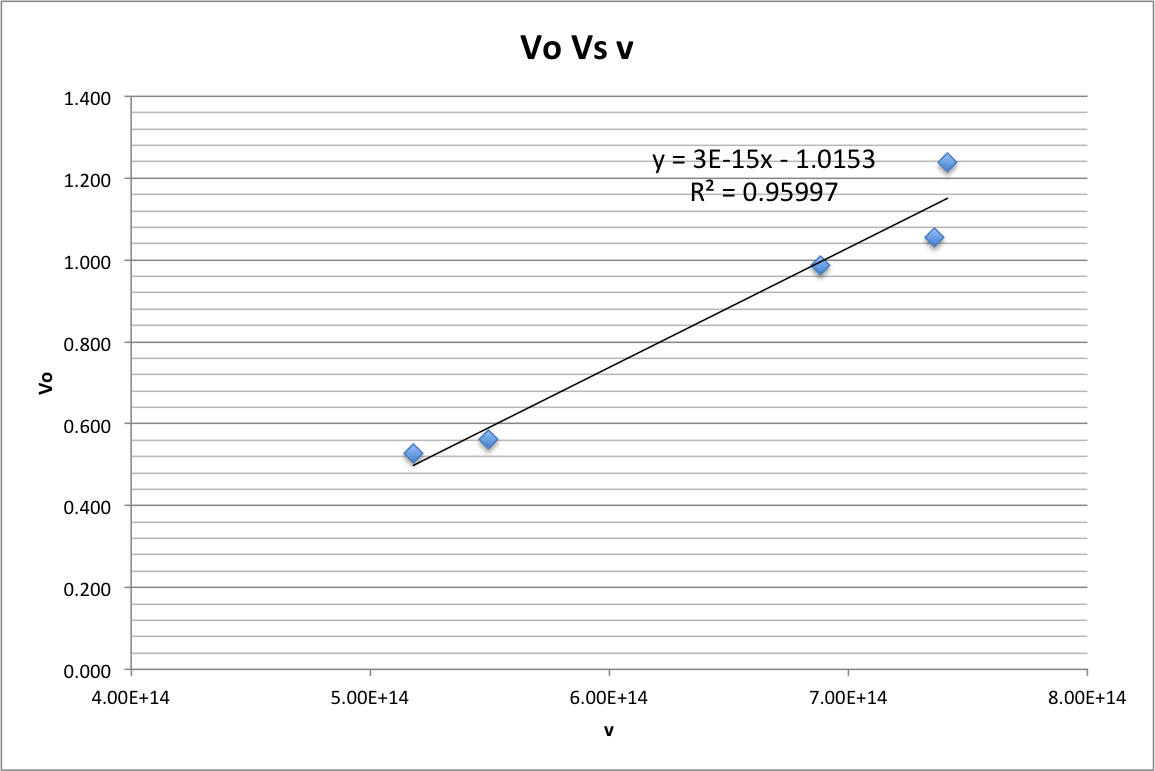
\includegraphics[width=0.75\textwidth]{33}
    \caption{Potencial de frenado $V_{0}$ en función de la frecuencia $\nu$.}
    \label{fig:my_label}
\end{figure}


    \item Encuentre la ecuación de la gráfica obtenida. Compárela con la ecuación $(8.4)$ determine de allí la constante $h$ de Planck. Recuerde que el valor de la carga del electrón es $1.60E-19 C$.
$\\$
$\bullet$ \textbf{Solución: }\newline
La ecuación obtenida de la gráfica es,
\begin{equation}
    y=3.0E-1514x-1.0153
\end{equation}
La ecuación $(8.4)$ nos dice despejando la variable dependiente $V_{0}$,
\begin{equation}
    V_{0}=\frac{h}{e}\nu-\frac{\omega_{0}}{e}
\end{equation}
donde $\nu$ es la variable independiente.\newline
Comparando con la ecuación de una linea recta se tiene que,
\begin{equation}
    y=mx\pm b
\end{equation}
donde $m$ es la pendiente de la recta, para nuestro caso se relacionada de la siguiente forma,
\begin{equation}
    m=\frac{h}{e}
\end{equation}
despejando y comparando se tiene y por último reemplazando los correspondientes valores de la carga del electrón se tiene
\begin{equation}
    h=e*m \ \longmapsto \ h=(1.60E-19 C)(3.0E-15 \frac{V}{s^{-1}})
\end{equation}
donde tenemos un valor de $h$ calculado,
\begin{equation}
    h=4.80E-34 Js
\end{equation}



    \item Compare el valor obtenido para $h$ con el valor teórico.
$\\$    
$\bullet$ \textbf{Solución: }\newline

Comparando el valor obtenido mediante la gráfica, determinamos un error porcentual.
\begin{equation}
    \%E=\frac{|6.625E-34 - 4.80E-34|Js}{6.625E-34 Js}\times 100\%=27.5471\%
\end{equation}

    \item De su gráfico determine la frecuencia umbral o de corte $\nu_{0}$, y la función de trabajo de la fotocelda $\omega_{0}$. Qué significado físico tienen $\nu_{0}$ y $\omega_{0}$
$\\$
$\bullet$ \textbf{Solución: }\newline

Para determinar la función de trabajo $\omega_{0}$ realizamos la siguiente comparación,
\begin{equation}
    b=\frac{-\omega_{0}}{e} \longmapsto \ \omega_{0}=-b*e
\end{equation}
\begin{equation}
    \omega_{0}=(1.0153 V)(1.60E-19 C)=1.62448E-19 J=1.01 eV
\end{equation}
y la frecuencia de corte $\nu_{0}$ se obtiene,
\begin{equation}
    \nu_{0}=\frac{\omega_{0}}{h}=\frac{1.62448E-19 J}{4.80E-34 Js}=3.38E+14 Hz
\end{equation}
la función de trabajo que es la mínima energía para extraer un electrón de la superficie del metal y depende del metal usado, los electrones extraídos del nivel de Fermic regresan hasta cierto punto y la corriente y el voltaje disminuye hasta un limite menor de cero.\newline
Cuando la energía cinética es cero, se tiene una frecuencia mínima  llamada frecuencia umbral, la cual es la frecuencia mínima desde donde empieza a presentarse el efecto fotoeléctrico.[3]
 
 
    \item Para el color amarillo grafique el potencial de frenado en función de la intensidad luminosa, representada por el filtro de transmisión. En el mismo gráfico haga lo propio para el color verde.
$\\$
$\bullet$ \textbf{Solución: }\newline

\begin{figure}[h!]
    \centering
    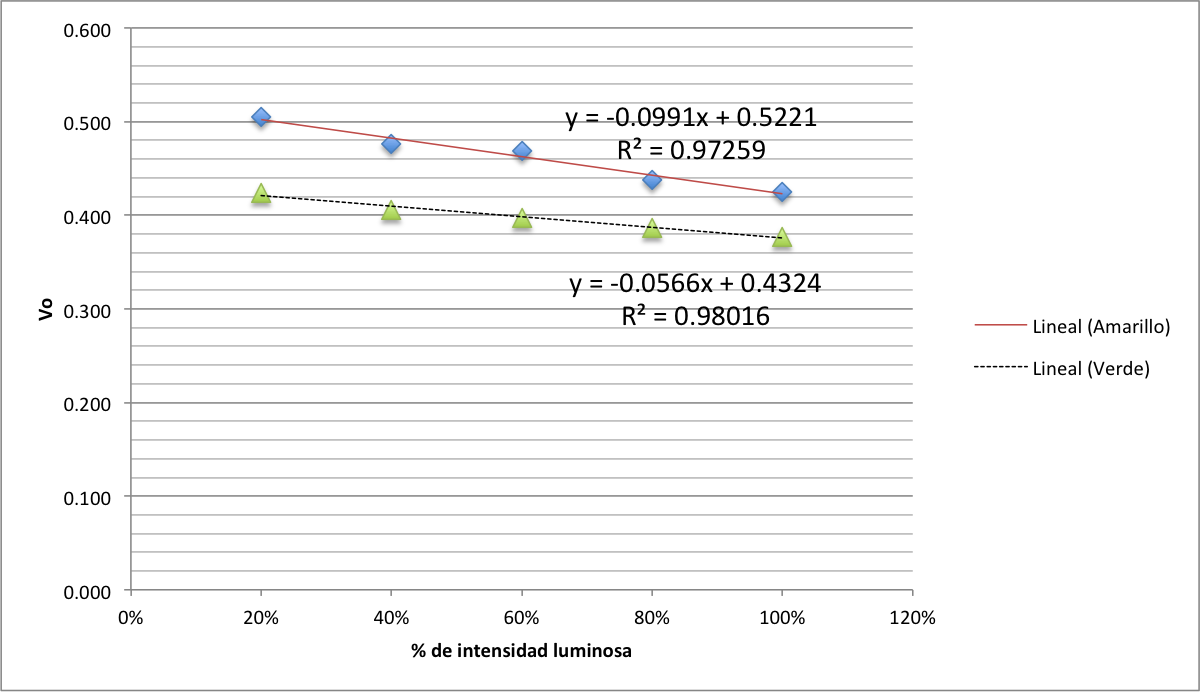
\includegraphics[width=0.78\textwidth]{2}
    \caption{Potencial de frenado $V_{0}$ en función de la intensidad luminosa, color amarillo y verde.}
    \label{fig:my_label}
\end{figure}

    \item Analizando el gráfico anterior: Depende el potencial de frenado de la intensidad luminosa?. Explique.
$\\$
$\bullet$ \textbf{Solución: }\newline

El potencial de frenado $V_{0}$ es independiente de la intensidad de luz incidente porque cuando se aumenta la intensidad de la luz, la corriente de saturación aumenta pero los electrones tienen la misma energía ya que el potencial de corte es el mismo.

    \item Discuta si sus resultados están mejor sustentados por un modelo cuántico de la luz o por un modelo ondulatorio.
$\\$
$\bullet$ \textbf{Solución: }\newline
Los resultados obtenidos se encuentran sustentados por el modelo corpuscular de la luz, donde la luz interactúa con la materia y se produce un intercambio de energía discreto, lo anterior fue descrito en la práctica partiendo de la obtención de la constante de Planck y relacionando las variables con la energía del fotoelectrón. 

    \item Consulte aplicaciones de las fotoceldas.
$\\$
$\bullet$ \textbf{Solución: }\newline    
\begin{enumerate}
    \item controlar el encendido automático del alumbrado público.
    \item alarmas.
    \item circuitos contadores electrónicos de objetos y personas.
\end{enumerate}


\section{Conclusiones}
\begin{enumerate}
    \item El número de fotoelectrones es proporcional a la intensidad de la luz incidente.
    \item La energía cinética máxima de los electrones depende de la frecuencia y no de la intensidad de la luz.
    \item El potencial de frenado  depende de la función de trabajo.
    \item Existe una frecuencia umbral  por debajo de la cual no ocurre el efecto.    
\end{enumerate}
    
\section{Bibliografía}
$\\$
[1] 
\ \ Medición de la carga del electrón (2012), Universidad Tecnológica de Pereira. Tomado de:\\ http://media.utp.edu.co/facultad-ciencias-basicas  /archivos/contenidos
-departamento-de-fisica/\\
experimento8if.pdf
$\\$
[2] 
\ \ Photoelectric effect, Colorado University, Tomado de: the Physics Hypertextbook \\ http://physics.info/photoelectric/
$\\$
[3] 
\ \ Medición de la carga del electrón (2012), Universidad Tecnológica de Pereira. Tomado de:\\ http://media.utp.edu.co/facultad-ciencias-basicas  /archivos/contenidos
-departamento-de-fisica/\\
experimento10if.pdf    
    
    
    
    
 
 
 
 
 
    
\end{enumerate}

\end{document}
